\section{Analysis of Algorithms}
{\tiny characterize running times of algorithms as a function of input size:\\
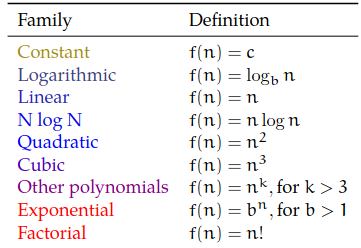
\includegraphics[scale=0.25]{functions.png}
}\\
\scriptsize{Logarithm} {\tiny the inverse of exponentiation: x = logb n -> b**x = n \\
for us, no base means base-2 \\
log xy = log x + log y \\
log (x/y) = log x - log y \\
log x**a = a log x \\
logb x = logk x / logk b\\
grow much slower than linear functions
}\\
\scriptsize{Polynomials} {\tiny degree-0: f(n) = c\\
degree-1: f(n)=n+c\\
degree-2: f(n)=n**2+n+c\\
generally drop the lower order terms\\
1+2+3+...+n = n(n+1)/2
}\\
\scriptsize{Permutations}\\ 
{\tiny n! = n*(n-1)*...*2*1\\
P(n,k) = n*(n-1)*...*(n-k-1) = n!/(n-k)!} \\
\scriptsize{Combinations}\\ 
{\tiny n choose k C(n,k) = P(n.k)/P(k,k) = n!/(n-k)!*k!\\
P(n,k) = n*(n-1)*...*(n-k-1) = n!/(n-k)!}\\
\scriptsize{Proof by induction}\\ 
{\tiny used for both proving the correctness and running times of algorithms\\
show that the base case holds\\
assume the result is correct for n, show that it also holds for n+1
}\\
\scriptsize{Hardware independence} {\tiny characterized by random access memory (RAM)\\
the data and instructions are stored in the RAM\\
processing unit performs basic operations in constant time\\
any memory cell with an address can be accessed in equal (constant) time\\
the processor fetches them as needed and executes following the instruction\\
there may be other, specialized registers\\
modern processing units also employ a cache
}\\
\scriptsize{Formal analysis of running time} {\tiny simply count the number of primitive operations\\
primitive operations include: assignment, arithmetic operations, compare primitive data types (in Java: boolean, byte, char, short, int, long, float and double), access a single memory location, function calls, return from functions\\
non-primitive operations: loops, recursion, compare sequences
}\\
\scriptsize{Big-O notation} {\tiny used for indicating an upper bound of an algorithm as a function of running time\\
if running time of an algorithm is O(f(n)), its running time grows proportional to f(n) as the input size n grows\\
drop the constants and lower order terms\\
transitivity: if f(n)=O(g(n)), and g(n)=O(h(n)), then f(n)=O(h(n))\\
additivity: if both f(n) and g(n) are O(h(n)), f(n)+g(n)=O(h(n))
}\\
\scriptsize{maximum problem size} {\tiny 
asymptotic analysis is important: assume we can solve a problem of size m in a given time on current hardware, when we get a better computer, we can calculate the new problem size we can solve in the same time\\
gap between polynomial and exponential algorithms: problem size for exponential algorithms does not scale with faster computers
}\\
\scriptsize{worst case analysis}\\ {\tiny in most cases we are interested in the worst case analysis \\
average case analysis is also useful, but requires defining a distribution over possible inputs and is often more challenging\\
pro: easier, get a very strong guarantee that the algorithm won't perform worse than the bound\\
con: in some problems, worst case examples are very rare
}\\
\scriptsize{asymptotic analysis}\\ {\tiny our analyses are based on asymptotic behavior \\
pro: correct for a 'large enough' input\\
con: constant or lower order factors are not always unimportant
}\\
\scriptsize{Big-O relatives} {\tiny Big-O(upper bound): f(n) is O(g(n)) if f(n) is asymptotically less than or equal to g(n)\\
Big-Omega (lower bound): f(n) is Omega(g(n)) if f(n) is asymptotically greater than or equal to g(n)\\
Big-Theta (upper/lower bound): f(n) is Theta(g(n)) if f(n) is asymptotically equal to g(n): f(n) is O(g(n)) and f(n) is Omega(g(n))
}\\
\scriptsize{Summary} {\tiny sublinear (e.g. logarithmic), linear, and nlogn algorithms are good\\
polynomial algorithms may be acceptable in many cases\\
exponential algorithms are bad
}